\chapter{Variable Range Hopping}		% chapter 3
\label{theorychap}

\section{Overview}
In order to understand our work with {\sc dias}, we must first go over a few seemingly disconnected topics. We begin by discussing the Monte Carlo method as it is the basis for our simulator. We then go on to discuss the physics of Coulomb glasses and how they relate to granular nanosolids. The point of this program is to simulate thermoelectric effects in granular nanosolids, so we will focus on thermoelectrics next. Finally we will be ready to dive into {\sc dias}.

\section{Monte Carlo methods}
Monte Carlo methods are a randomized way to use the law of large numbers to find answers to mathematical and physical problems. For example, In oil and space exploration, Monte Carlo methods are a better predictor of cost overruns than human intuition~\cite{Hubbard09}. While there is no consensus on the exact definition of a Monte Carlo method, One can get a feel for it by looking at simple examples. Some good examples are the estimation of $\pi$ and the Metropolis method.

\subsection{Estimating $\pi$}
Estimating $\pi$ has been a challenge for mathematicians since ancient Egyptian times. One possible method is by trying a Monte Carlo strategy. For simplification, one usually just takes a fourth of a circle inscribed in a square (see fig.~\ref{piSquare}). One then picks random numbers between 0 and 1 for x and y. Success is then defined as ~\cite{Kalos08}:
\begin{eqnarray}
\sqrt{x^2 + y^2} < 1 .
\label{piSuccess}
\end{eqnarray}
In a way, all we are doing is integration. If one counts the number of successes and divides by the number of total trials, it will equal to the ratio of the area of the quarter circle and the square of length 1, which can then be solved for $\pi$. Integration of this sort can be used to approximate the area under any integrable curve, and in the case of the "pathological equation" some non-integrable ones as well~\cite{Newmann99}.

\subsection{Metropolis method}
The Metropolis algorithm is a way to draw samples from a probability distribution iteratively. Because each distribution is only affected by the previous distribution, this can be considered a Markov chain. A Markov chain is a sequence of random variables which a system moves through with serial dependence. In its simplest sense, we have
\begin{eqnarray}
\overrightarrow X_{t+1} = \overrightarrow{ \overrightarrow Q} \overrightarrow X_{t} ,
\label{Markov}
\end{eqnarray}
where $\overrightarrow X_t$ is the state of the system at step $t$, and $\overrightarrow{\overrightarrow Q}$ is the probability matrix. Under certain circumstances, the probability matrix can be applied multiple times, eventually causing the state to approximate an equilibrium~\cite{Everitt02}. The Metropolis method can be used for many systems, but we will focus on the Ising problem as it is similar to our problem.

\subsection{Ising problem}
The Ising method is a way to solve the problem of dipole moments on a large array of atoms. While the Hamiltonian can be fairly straightforward (see Eq.~\ref{Ising}), its properties such as its specific heat or hysteresis can be relatively complex.
The Hamiltonian is
\begin{eqnarray}
H(\sigma) = - \Sigma J_{ij} \sigma_i \sigma_j - \mu \Sigma h_j \sigma_j , 
\label{Ising}
\end{eqnarray}
where $\sigma_i$ is the spin, $J_{ij}$ is the interaction strength between neighbors, $\mu$ is the magnetic moment, and $h_j$ is an external magnetic field. Then the configuration probability is:
\begin{eqnarray}
P(\sigma) = \frac {e^{-\beta H(\sigma) }} {Z_\beta },
\label{configurationProbability}
\end{eqnarray}
where $\beta = (k_B T)^{-1}$, and the renormalization constant $Z_\beta = \Sigma e^{-\beta H(\sigma)}$. From here we have a 3 step process to simulate the system. First, we must choose an arbitrary configuration to be our starting point. Next, we pick an adjacent configuration in configuration space (i.e. a configuration that we can get to by just changing one value). If going there is energy favorable, then the change is made. Otherwise, the change is made depending on the temperature. As the system is evolved, variables such as magnetic field and temperature can be changed, which can lead to properties such as specific heat and hysteresis. 

	Calculating the partition function (Eq.~\ref{configurationProbability}) in the thermodynamic limit involves doing an infinite amount of sums. The first step to simplifying this is to approximate the system on a lattice of finite size. Because of the dynamic complexity of even a small system (a 10 by 10 system can have $2^{100}$ configurations) simulations are a large part of modern electron hopping studies ~\cite{kirkengen09}. If we could sample $2^{45}$ of those sites on a good computer in a few hours, we would still miss out on the vast majority of states. This problem would be made worse at low temperatures where the system is dominated by a handful of ground states. Using a Monte Carlo system, we can find out which states will make important contributions to Eq.~\ref{configurationProbability}. There are however imporant conditions which must be followed when crafting a Monte Carlo system.

\subsection{Conditions}
There are certain conditions which an algorithm must comply with in order to be considered a Markov Chain Monte Carlo. The first is that the probability function should not vary over time. That is clearly satisfied as we stay in the form:

\begin{eqnarray}
P = e^{-2R - \Delta E/T},
\label{simpleProb}
\end{eqnarray}
where the probability of jumping is a function of the jump distance $r$, change in energy of the system $E$, and temperature of the jump site $T$. The second is that the probability to jump to the next state is only a function of the current state. In other words, there is no "momentum" built up from previous states. Third is that the sum of the probabilities must equal 1:
\begin{eqnarray}
\Sigma P(\mu \rightarrow \nu) = 1 ,
\label{normalized}
\end{eqnarray}
Where $\mu$ is the current state and this is being summed over all possible transitions to other states $\nu$. Fourth is the requirement of ergodicity. That is, all states should be reachable from all other states given enough time. This requirement is satisified as long as there is at least one non-zero probability to jump out of every other state. Finally, our last condition is of detailed balance. That is, upon relaxation we generate the Boltzmann probability distribution rather than any other.

Kinetic Monte Carlo methods are useful when simulating condensed matter systems which include time evolution. There are two types, rejection and rejection-free, the difference being whether or not an event has a chance of failing all-together. If a kinetic Monte Carlo method is also subject to detailed balance, then it simulates a system at thermodynamic equilibrium~\cite{Young66}. A kinetic Monte Carlo method is useful for modeling variable range hopping. The temperature dependence of conductivity can be tested using a kinetic Monte Carlo algorithm.

\section{Coulomb Glass}
In 1937, Nevill Mott and Rudolf Peierls explained why some materials which should have been conductors, acted as insulators. This was due to electron-electron interactions, which is not taken into account in band theory ~\cite{mott72}. From there, Miller and Abrahams proposed a network resistor model which Efros and Shklovskii built on ~\cite{efros75}. The theory has gotten more consise over time. For the sake of simulation, much of it can be compressed into equation~\ref{probability}.

Transport through a quantum dot which is weakly coupled to two conducting leads is dominated by the electron-electron interaction ~\cite{Glazman05}. When the thermal energy is not enough to overcome the charging energy of the dot, Coulomb blockade takes over and resistance is increased. At low enough temperatures, the Kondo effect takes over. That is when the magnetic field of the electrons starts to matter energy-wise. At that point, electrons start to prefer states where they are anti-parallel.

If one assumes that single-particle excitations are responsible for variable range hopping, then one ends up with the Efros-Shklovskii law:
\begin{eqnarray}
\sigma_c \approx (\gamma e^2 / T) \exp(-(T_0/T)^{1/2}),
\label{ESlaw }
\end{eqnarray}
Where $\sigma_c$ is the conductivity, $\gamma$ is the frequency, $T$ is the temperature, and $T_M = \beta_M (g_0 a^2)^{-1}$ where $a$ is the localization length of the electron, $g_0$ is the density of states at the Fermi level, and $\beta_M$ is a numerical coefficient.~\cite{Tsigankov02} show that single electron jumps are sufficient to describe the system. This is important since otherwise we would have to simulate multi-electron jumps which would scale the difficulty of simulation by an order of magnitude. The problem of studying this situation increases with decreasing temperature as electrons are able to jump farther. 

The Coulomb glass system was found to be robust enough to relax within simulateable times. ~\cite{Kirkengen09} Found that the relaxation time is slightly slower than exponential. Energy correlations at equilibrium however were found to be exponential:
\begin{eqnarray}
C(\tau) = e^{-(\tau / \tau_0)^\gamma},
\label{correlations}
\end{eqnarray}
where $\gamma$ is proportional to temperature at low temperatures, and $\tau , \tau_0$ are time dependent. Only at low temperatures below $T_{min} \approx 0.02$ does the system take too long to equilibrate. The behavior is similar to that of a random walk on a fractal configuration space. 

The Coulomb glass is applicable to nanoscale nanular lattices, and much research has been conducted on them. Abeles et. al. did some of the original work on nano-granules. They achieved this by co-sputtering metals and insulators. They attributed conduction due to electron percolation and tunneling. They also define a charging energy required to tunnel as $E_j = e^2/2C$ where $C$ is an effective junction capacity. Another interesting phenomenon that they observed was that of the electric field breakdown. That is, if the voltage drop between particles became comparable to the height of the tunneling barrier, then electrons could go straight into the conduction band of the insulator. 

In ~\cite{Vinokur08} The 2D lattice of Coulomb glasses with site disorder was studied. When the effect of site disorder was on the same scale as the Coulomb energy, the distribution of local minima becomes exponential. At low disorder, the density of states becomes crystal-like. They also found that in order to fully relax a system, multiple-electron jumps must be taken into account. 

\subsection{Density of States in a Coulomb Glass}
There are many methods of characterizing the energy of an electron. One of these is the density of states. This is a histogram of the energies that electrons can be in. For example in ~\ref{moundDoS}, there are many electrons at a relatively low energy and the number of electrons with higher energies decreases with energy. In ~\ref{crystalDoS} there is only one energy option for electrons. We see two peaks because the holes act as particles in that the system requires energy to move those as well. The value on the x axis is the energy required to fill or empty each hole or particle respectively. By knowing the shape of the density of states, one can discern important intricacies of a system. These can include the energy scales, the relaxedness, and the bandgap of a system. If the particle distribution is symmetric (same amount of electrons as holes) then the density of states will be symmetric, as long as the system is relaxed~\cite{Kittel96}.

\begin{figure}[htbp]
\begin{center}
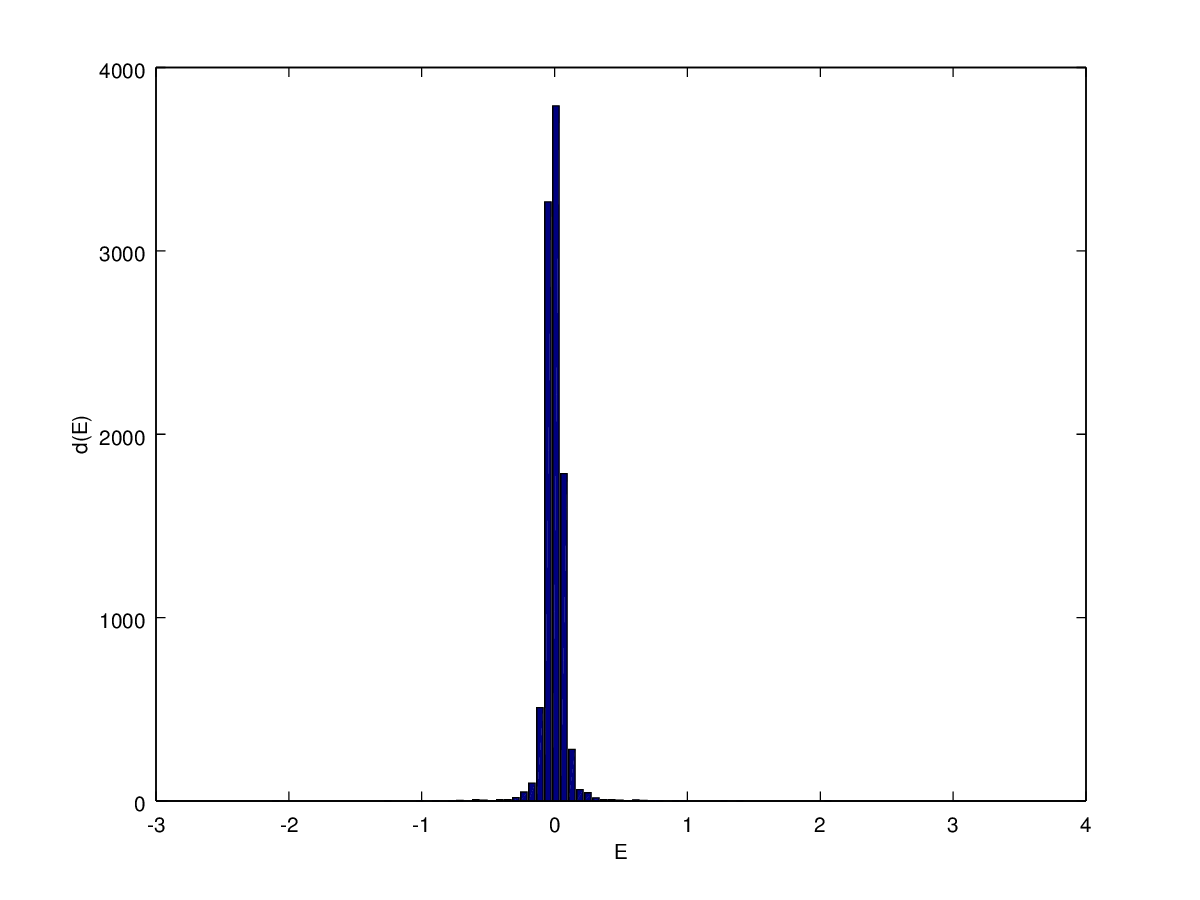
\includegraphics[scale=.50]{veryCloseDos.png}
\caption{The density of states for a system with a high amount of randomness in the energy.}
\label{moundDoS}
\end{center}
\end{figure}

\begin{figure}[htbp]
\begin{center}
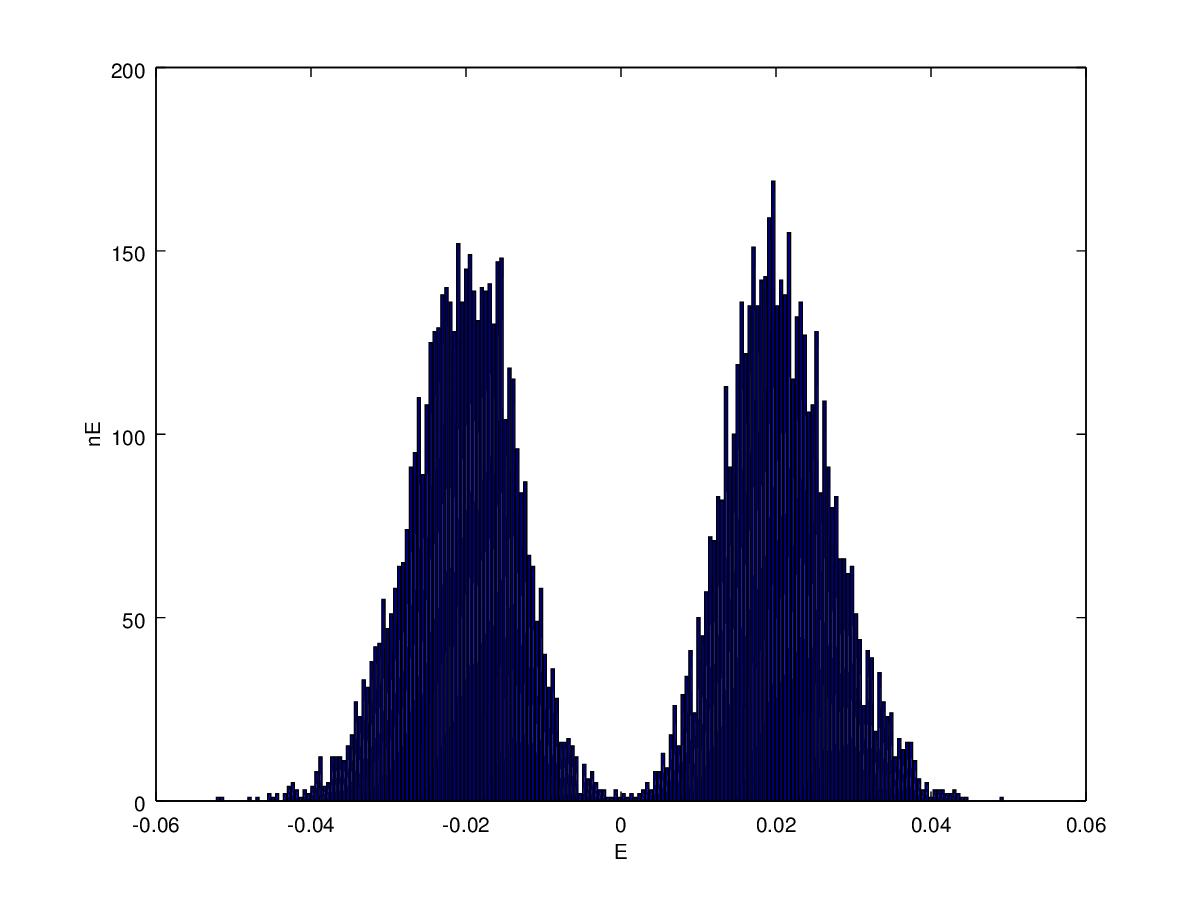
\includegraphics[scale=.50]{critDoS.png}
\caption{The density of states for a system where there is a critical amount of randomization and the two peaks are just beginning to touch.}
\label{critDoS}
\end{center}
\end{figure}


\begin{figure}[htbp]
\begin{center}
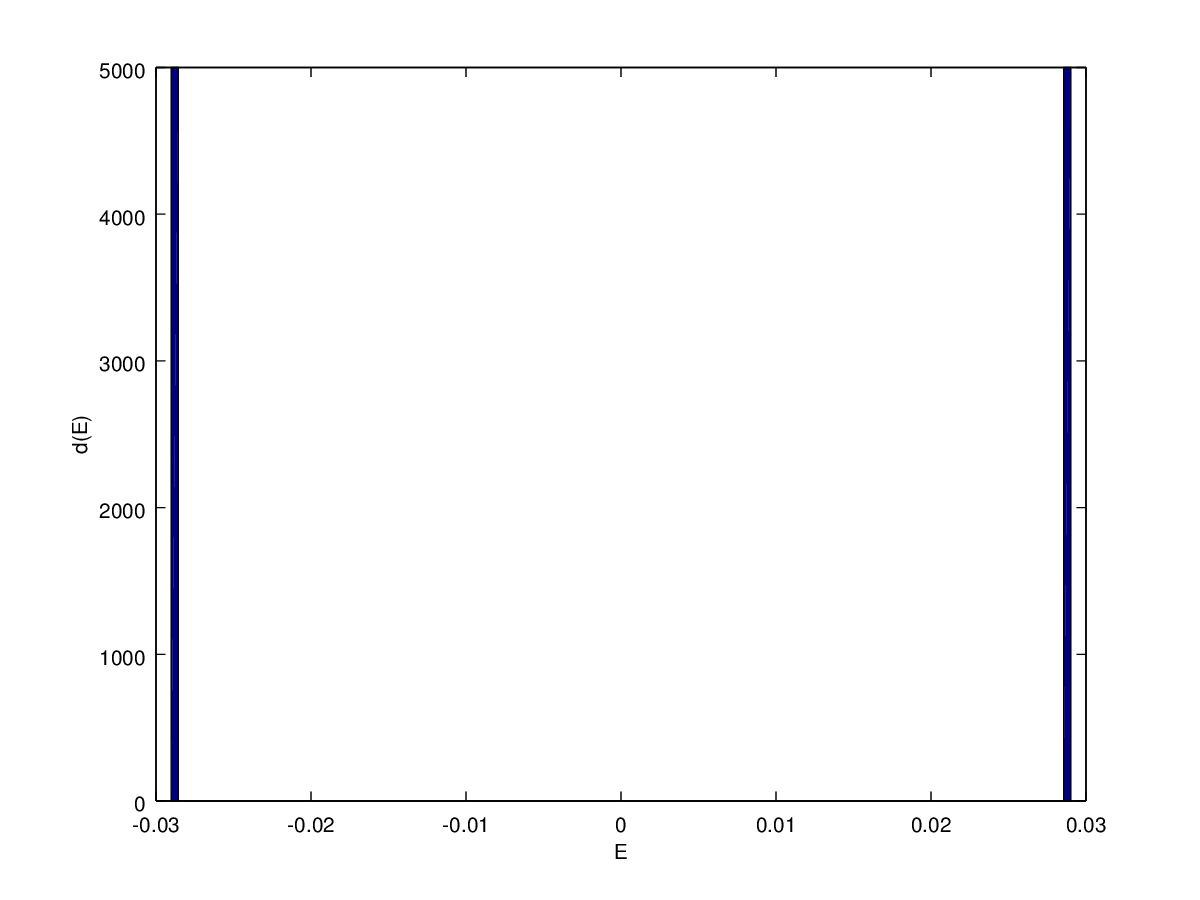
\includegraphics[scale=.50]{splitDos.png}
\caption{A low entropy system (Wigner crystal).}
\label{crystalDoS}
\end{center}
\end{figure}

\subsection{Comparing Mott VRH against Effros-Shklovskii VRH}
While the approach to describe physical systems by Mott vs Effros-Shklovskii (ES) theory are similar, there are a few key differences in the details. First, The localization parameters are different due to differences in the density of states. The localization is temperature dependent in the ES system. This is because ES considered the situation where if an electron tries to tunnel, It must leave an electron hole behind. This enhanced requirement for the energy means that at low temperatures, the density of states at the Fermi level vanishes ~\cite{joung}. The resistivity for the Mott system ends up being related to the temperature as

\begin{eqnarray}
\ln(\rho) \approx (T_o / T)^{1/4} ,
\label{fourth}
\end{eqnarray}
where $\rho$ is the resistivity and $T$ is the temperature. Meanwhile, in the ES system we have
\begin{eqnarray}
\ln(\rho) \approx (T_o / T)^{1/2}.
\label{half}
\end{eqnarray}
The Mott resistance comes from $\delta E = \alpha_1 / g r_{ij}^3 $, where $\alpha_i$ are prefactors of order unity. The ES resistance comes from the usual Coulomb blockade term $\delta E = \alpha_2 e^2 / \kappa r_{ij}$ ~\cite{aharony92}. The Differences can be summarized in a single plot ~\ref{MvsES} ~\cite{Liu10}.

\begin{figure}[htbp]
\begin{center}
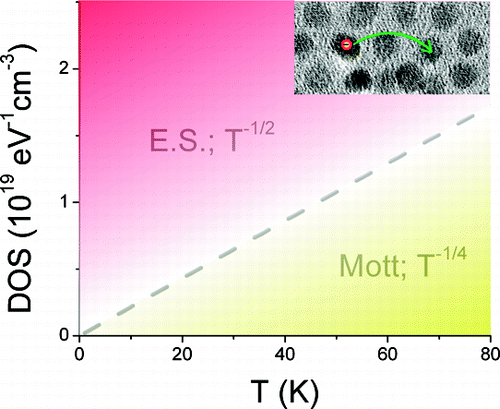
\includegraphics[scale=.50]{MottvsES.png}
\caption{Density of states vs Temperature. This plot describes the interface between ES and Mott transmission of electrons. (Graph courtesy of Heng Liu)}
\label{MvsES}
\end{center}
\end{figure}


\section{Artificial Nanosolids}

In a sense, artificial nanosolids are like hyper-Coulomb glasses. They have many of the same attributes if one treats each atom as a granule. Each granule consists of thousands of atoms, yet is small enough to observe the Coulomb blockade. They are also known as granular films and can be prepared by co-sputtering metals such as nickel and gold with insulators such as silicon dioxide or aluminum oxide. Strong electron scattering from dielectric inclusions or grain boundaries. Electrical transport will typically occur via tunneling between granules. Intra-grain conduction is significantly higher than inter-grain conduction and so is typically ignored. Depending on the type of material (conductors, semiconductors, insulator), the energy levels inside the granules can be tuned. The size of the granules also plays a large role in determining the energy levels~\cite{Abeles75}.  These metallic particles act like artificial atoms with programable electronic properties. These can be formed such that they are insulators, conductors, semiconductors, or even superconductors. Beloborodov et. al.~\cite{Beloborodov07}  Were able to show that there was logarithmic temperature dependence of the conductivity. This system also appears to show negative magnetoresistance under certain parameters. 

By tuning the ability of electrons to travel, one can also start to change the Seebeck coefficient of the material~\cite{Glatz09}. The Seebeck coefficient gives us a general idea of the performance of the artificial nanosolid. Glatz et. al. derive the thermopower and thermoelectric coefficient of nanogranular materials. They find the thermoelectric coefficient to be:
\begin{eqnarray}
\eta = \eta^{(0)} (1 - \frac{1} {4 g_T d} ln \frac{g_T E_c} {T} ),
\label{thermoelectric}
\end{eqnarray}
where $\eta^{(0)} = -(\pi^2 / 3) e g_T a^{2-d} (T/ \epsilon_F)$, $a$ is the size of a grain, $d$ is the dimensionality of the system, $\epsilon_F$ is the Fermi energy, and $E_c = e^2 /a$ is the charging energy.

\subsection{Inelastic vs. Elastic tunneling}
As well as blocking each other, electrons also can impart energy onto each other which may result in an electron being dislodged. This is referred to as inelastic co-tunneling. If instead the electron tunnels or otherwise travels without dislodging, it is referred to as elastic co-tunneling (see fig. ~\ref{inelasticvselastic}). For low to medium temperatures, the main tunneling mechanism will be elastic. At higher temperatures, we expect a transition to in-elastic tunneling~\cite{Glazman05}.

\begin{figure}[htbp]
\begin{center}
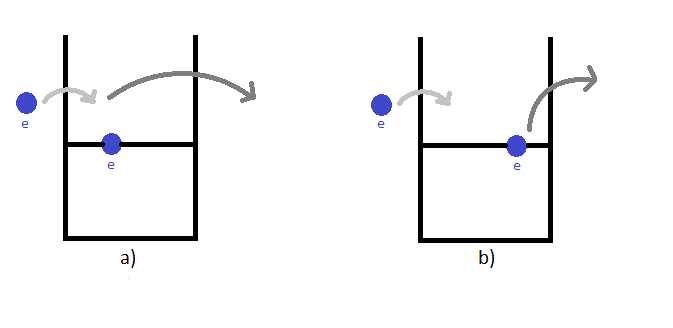
\includegraphics[scale=.50]{inelasticvselastic.png}
\caption{a) elastic transmission of electrons. b) inelastic transmission of electrons.}
\label{inelasticvselastic}
\end{center}
\end{figure}


\subsection{Coulomb Glass vs Artificial Nanosolids}
Coulomb glasses are the original substrate on which the ES model of electron conduction was based. The "glass" in Coulomb glass refers to a phase in which electron-electron interactions impair conduction and dynamics become slow, like the flow of a glass~\cite{ortuno04}. Artificial nanosolids are arrays of granules which have a higher intra-granule conduction than a inter-granule conduction. The differences begin at the density of states. In artificial nanosolids, the density of states can be more creative. By changing the size of the granule, and the material it is made out of (metal, insulator, superconductor) the amount of available electron slots per site (and the energy of each slot) can be chosen. There are two energy scales for each grain. $\delta$ is the mean level spacing. $E_c$, the energy required to pack on one more electron onto a site is on the order of 3000 Kelvin ~\cite{glatz08} .The distances are also different. For Coulomb glasses, the distances are basically the inter-atomic distances. There we are basically talking about electron jumps between atoms on a crystal lattice. As the name suggests, in artificial nanosolids the distances are nanoscale and tuneable. For typical artificial nanosolid applications, we are in the nanometer to tens of nanometers range~\cite{beloborodov05}. While the general electric potential plays a role in both systems, It plays a bigger role in the Coulomb glass since the scales are smaller and the electric potential scales as $1/r$. Before we get too far into the practical applications of artificial nanosolids, we must first discuss thermoelectrics.


\section{Thermoelectrics}
Thermoelectric devices are a way to get electrical energy out of thermal gradients or vice versa. The problem is that electrons which conduct electricity also conduct most of the heat. Materials which tend to be good electrical conductors also tend to be good thermal conductors. This conundrum is refered to as the Wiedemann-Franz law~\cite{glatz09}. 

	There are two governing variables in thermoelectrics, device efficiency and power factor. 
\begin{eqnarray}
\eta = \frac{E_{in}}{E_{W}},
\label{efficiency}
\end{eqnarray}
where $E_{in}$ is the energy put into the system, and $E_{W}$ is the heat pumped to the hot end. The power factor for a thermoelectric is:
\begin{eqnarray}
P = \sigma S^2,
\label{power}
\end{eqnarray}
where $\sigma$ is the conductivity.

 The number that denotes usefulness of a thermoelectric device is the dimensionless figure of merit
\begin{eqnarray}
ZT = \frac{\sigma S^2 T}{k},
\label{ZT}
\end{eqnarray}
where $\sigma$ is the conductivity, $S$ is the Seebeck coefficient, $T$ is the temperature, and $k$ is the thermal conductivity ~\cite{chen}. The Seebeck coefficient is a relationship between the electric gradient and the thermal gradient:
\begin{eqnarray}
S = \frac{V}{\Delta T},
\label{Seebeck}
\end{eqnarray}

In order to have optimal conditions, phonons must see the substrate as a glass, while electrons see it as a crystal~\cite{Rowe05}. Each granule in the Coulomb glass-like material acts to scatter phonons. If a semiconductive lattice of granules is interspersed with conductive granules, then tunneling electrons will effectively see a crystal. With this understanding of the physics involved, we wrote {\sc dias}.  

\section{{\sc dias}}

\subsection{Algorithm Parameters and Choices}
{\sc dias} (Dynamics In Artificial Solids) is a code which at its heart is a 2D Monte-Carlo simulator. {\sc dias} begins by taking in parameters such as granule-to-granule distance, number of electrons, number of lattice sites, number of time-steps, temperature, voltage bias, thermal gradient, material coefficient, and substrate potential variance. The granule-to-granule distance is on the order of 10 nanometeres. We have a square grid which is periodic. Variances in granule distances are uniformly introduced with limits according to user-set parameters. The number of electrons can vary between double-empty systems and double occupied sites. The number of time-steps is usually set to the square of the number of particles. This is to ensure a statistically justified result from the monte carlo aspect of the simulation. Temperature is set in Kelvin and is usually varied in the range where our material coefficient would give interesting results.  A positive voltage bias will act on a particle so that it is coerced to move upstream. Conversely, a positive voltage bias will force a hole to move downstream. This hints at a particular symmetry in which we chose for the simulation. Some previous studies have chosen to only focus on electron jumps and reject any jump that begins with a hole ~\cite{Ferrero14}. We decided to allow jump probabilities to be calculated from an electron hole's point of view as well. For current/voltage measurements, the system is periodic so that the current will just keep traveling at a steady pace. A second version of the code was created where the boundaries formed a closed system to study thermoelectric properties. The memory choices we made are also worth mentioning. There were several arrays of data and keeping these to a minimum was important as memory management was an issue due to the limited space on GPU cards. These matrices include particle/hole, substrate potential, distance between sites, thermal gradient, and size of each granule. In order to maintain neutrality, the voltage bias was artificially set. This meant that the effective charge of a filled site was half an electron. If an electron were to move, the charge then became negative half and electron. The Monte-Carlo algorithm shows up twice to find the jump site.  

\subsection{Algorithmic Strategy}
First, a lattice site is chosen with probability according to its energy. Second, the jump probabilities to each site are calculated using Eq.~\ref{probability} for said site. We do not allow jump probabilities greater than $L/2$. In fact, the system is periodic, so anything past $L/2$, is actually closer than $L/2$ in the other direction. These probabilities are summed up and a number is chosen between 0 and that sum. This in turn gives a Monte-Carlo jump which is weighted by the jump probabilities. This jump is done and the system moves on to the next timestep under the new electron configuration. Meanwhile the properties of interest are measured. This repeats for the number of requested time steps. Originally we picked the starting particle randomly. Unfortunately in order to have a rejection-less system, this cannot happen. If it did, then particles which would have practically no chance of jumping would be moved with probability $ 1/N^2$, the same as any other particle. In order to fix this, we followed the algorithm posed in ~\cite{Newman99}. They propose first picking two particles with probabilities via the tower method, based on their energies. This way, particles which are less stable are moved more often. Because of the distance parameter in our probability, we are forced to pick one particle at a time. This way the second particle is picked based on the change of energy of the system, with a distance component. This algorithm allows for maximum parallelization and no rejection. The parallelized tower method is efficient as we can use a parallel prefix scan to stack the probabilities while also finding the maximum value in order to normalize. Doing a search for the right interval can also occur in parallel as each thread can be given a range, and the appropriate range can be found in log(N) time.

\subsection{GPU Algorithms}
Electron hopping via Monte-Carlo algorithm can be solved particularly efficiently using parallel/GPU algorithms. Specifically we use an algorithm called the "tower method" ~\cite{Krauth06}. Typically when one is doing a Monte Carlo study, there is an acceptance region and a rejection region ammong a range of choices. A choice is examined and it is either rejected or accepted. Using the tower method, all choices are stacked on top of each other (like a tower) and there is no rejection region. The first step, finding the probability to jump to each site is solved via the classical parallel scheme, where each lattice site can be individually calculated in its own thread. Once we have the probability matrix, we need to sum it in order to normalize it. This can be done via a parallel reduction algorithm. Taking advantage of on-board GPU memory, we can perform the reduction in O(N/P + log N ) time rather than O(N) time, where P is the number of GPU cores. Now that the system is normalized, we can roll a dice between 0 and 1 to find where the particle will go. We must then sum our probabilities until we find that number. This can be done with a parallel prefix sum. Parallel reduction and prefix sum algorithms were written and then replaced by Nvidia's more efficient Thrust functions. Thrust is a template library for CUDA which allows the implementation of high performance parallel applications. Each choice of substrate and position randomization has its own ground state. This ground state is found through a relaxation algorithm.






\begin{varwidth}{\dimexpr\linewidth-2\fboxsep-2\fboxrule\relax}
\begin{algorithmic}[1]
\State First a nearest neighbor exchange
\For {n = 1 to number of sites}
\If {there's a particle at that site}
\State calculate energy without moving the particle:
\State {\textit{potential energy calculated everywhere}}
\State {\textit{sum reduction of the potential energy to one number (lets call it $S_1$) }}
\State test moving the particle up
\State {\textit{potential energy calculated everywhere}}
\State {\textit{sum reduction of the potential energy to one number (lets call it $S_2$) }}
\If {$S_1$ $>$ $S_2$}
\State leave the system
\Else
\State change it back
\EndIf
\State repeat for the other 3 directions (down,left,right)
\EndIf
\EndFor
\State The system is now slightly more relaxed
\State Now for switching highs and lows
\While {system is not relaxed}
\For {n = 1 to number of sites}
\State find the energy at each site normally:
\State {\textit{calculate potential,substrate, \& coulomb blockade energy everywhere. Sum and call this $S_3$}}
\State find the energy at each site with the particle removed (or added if the site was empty ):
\State {\textit{calculate potential,substrate, \& coulomb blockade energy everywhere. Sum and call this $S_4$}}
\State DosMatrix[n] = $S_4$ - $S_3$
\EndFor
\State {\textit{find lowest and highest values on the DosMatrix}}
\If {DosMatrix[index of lowest] + DosMatrix[index of highest] $<$ 0 }
\State swap particles
\Else
\State system is relaxed
\EndIf
\EndWhile



This algorithm was previously used in ~\cite{glatz08}. 

\end{algorithmic}
\end{varwidth}%

Another part of this algorithm that is important to understand is the "Tower Method" and is integral to a kinetic Monte Carlo algorithm. It is used in picking the starting particle as well as picking the particle to jump to.







\begin{varwidth}{\dimexpr\linewidth-2\fboxsep-2\fboxrule\relax}
\begin{algorithmic}[1]
\State Total = 0
\For {n = 1 to number of sites}
\State Total =+ $P_n$
\EndFor
\State newSum = 0
\State pick a random number R from 0 to Total
\For {n = 1 to number of sites}
\State newSum =+ $P_n$
\If {newSum $>$ R}
\State stop For loop, current i is the jump site
\EndIf
\EndFor




Another way of thinking about this is by spinning a "wheel of fortune" style wheel where each slice's size is proportional to the probability.
\end{algorithmic}
\end{varwidth}%

The following pseudocode is what is referred to as the "Parallel Reduction". It is device specific to GPGPU's, but can be generalized depending on "shared memory". If generalizing, the maximum number for "shared memory" is equal to the number of processors available. This can be easily combined with a simple parallel sum to create a parallel dot-product algorithm. A similar algorithm can be used to efficiently determine the maximum or minimum number of each array. This time instead of placing the sum of the two numbers, one can place the larger of the two numbers. This algorithm can repeat until the largest number is found.








\begin{varwidth}{\dimexpr\linewidth-2\fboxsep-2\fboxrule\relax}
\begin{algorithmic}[1]
\State number of slices = sizeArray/sharedMemory + 1
\State size of slice = sharedMemory
\State sumStart = 1
\For {i = 1 to number of slices}
\For {k = 1 to log(size of slice)}
\For { j = sumStart to size of slice/2}
\State add first half of slice to second half, put that sum in the second half
\EndFor
\State sumStart = size of slice/2
\State size of slice  = size of slice / 2
\EndFor
\EndFor
\State (now we stitch each shared memory together)
\State totalSum = 0
\For {i = 1 to number of slices}
\State totalSum = totalSum + sliceSum
\EndFor




Many parallelized algorithms tend to take a "power of 2" strategy.
\end{algorithmic}
\end{varwidth}%



\subsection{Jump Probability}

In order to calculate the electron variable range hopping (VRH), we must first find the probability of each jump site. Our main equation involved is as follows:
\begin{eqnarray}
P_{ij} = \exp (-2\alpha R_{ij} -  E_{ij}/kT)
\label{probability}
\end{eqnarray}

where $k$ is the Boltzmann constant, $R_{ij}$ is the distance between cells, $E_{ij}$ is the energy change of the system if a particle were to move from i to j, and T is the temperature of the system.$\alpha = \sqrt{2mH/\hbar}$ where $m$ is the effective mass at the bottom of the conduction band and $H$ is the mean energy of the conduction band. $\alpha$ is set up to be around the same scale as the inter-grain distance. $E_{ij}$ has various inputs which vary in energy scale~\cite{Mott68}.
\begin{eqnarray}
E_{ij} =  \triangle U_{ij} e^2/a\kappa_1  + e f_i \triangle V_{ij} + f_i  \triangle \mu_{ij} + f_i (eV) \triangle x_{ij} 
\label{deltaE}
\end{eqnarray}
where $i$ refers to the starting site index and $j$ refers to the target site index,  $f$ is the occupation of a site, $a$ is the size of the granule, $\kappa_1$ is the intra-granule dielectric constant, $\mu$ is the substrate potential, $V_{ij} = \sum_{i,j=1}^{N} e^2/\kappa_2 r_{ij}$ is the local potential from the rest of the particles, $\kappa_2$ is the inter-granule dielectric constant, $\triangle x$ is the component of r in the direction of eV , and $eV$ is an externally applied voltage. $\triangle U_{ij}$ is the difference in charging energy. The first two components of equation ~\ref{deltaE} together constitute the electrostatic component of this system. The most powerful is the Coulomb blockade. This introduces a large penalty into the probability of an electron occupying the same site as another electron. If the site at which an electron can travel to is empty, the chances of transport are higher than if the site is filled ~\cite{glazman05}. There is also a contribution from the substrate. There is an inherent randomness in the potential at different lattice sites and that is where this comes in. This energy landscape somewhat randomizes starting energies and can fill in as electron donor. There is a general electric potential which will try to get the electrons to space out evenly in the substrate (periodic boundary conditions). Finally there is a current portion which if a voltage bias is applied on the left and right sides of the system, then the probability of electrons hopping with that bias is increased ~\cite{aharony92}. The exponential term is artificially limited below 0 to keep the electron hop ranges realistic. Analytically, equation~\ref{probability} can be maximized to find the most common jump distance (take the derivative with respect to r and set equal to 0). In our case, there are 2 problems with this approach. First, we are more interested in the average jump distance which need not be the maximum. Second, The analytical approach assumes a continuous system, where in reality it is a discrete number of interacting points.

\subsection{Optimizations}
Various optimizations were done in order to speed up this code. Originally this was a linear CPU code, but obvious parallelisms made this code perfect for being run on a GPU. Still, there were some less obvious optimizations. One such optimization was previously discussed, moving to a rejection free system. In a rejection system, the particle has a high chance of staying at the same cell each turn. This means that a lot of computation is spent not gaining any valuable information. To fix this, we moved to the rejection free system (BLK?)~\cite{Newman99}. It is as if one jumped the simulation forward skipping all non-events. For one to do this, the system time must be kept. This is done by integrating all of the probabilities:
\begin{eqnarray}
\delta t = \frac {1} {\Sigma P_{\mu \rightarrow \nu}},
\label{systemTime}
\end{eqnarray}
where $\delta t$ is the change in system time, and $P_{\mu \rightarrow \nu}$ is the Markov transition matrix. Because of {\sc cuda} and algorithms like parallel reductions, it ends up being much faster to calculate this than to try to calculate all of the rejections. There were optimizations that skipped unnecessary calculations. One of these was the calculation of the potentials after a particle is moved. The naive way to do this would be to recalulate all of the potentials from each particle. The optimized way to do this would be to use a crater-mound system. That is, only focus on the effects due to the particle that has moved. In other words, calculate the difference on the potential that taking that one particle away would change and calculate the sum on the potential that adding a particle would cause. Using a 4D lattice matrix also saved simulation time at the expense of system memory. This matrix held the distances of every particle with respect to every other particle. Technically this matrix only had to be $N^4/2$ in size, but making it $N^4$ simplified the already ardous task of using a 4D matrix and was faster than an algorithm which could operate on a $N^4/2$ matrix.

\subsection{The Lattice}
While the easiest system to model would have been a square lattice, This would have left out a large amount of interesting phenomena. To incorporate this, we started out with a square lattice and then gave each site a certain $\delta x$ or $\delta y$ variance. There are a few ways to then use this kind of implementation. The first one would have been to then calculate the distances from one site to another on the fly, possibly approximating for further away site. The way that we picked to do this was to hold all of the distances from one site to another in a 4D matrix (a matrix of distances for every site on the grid). This has the advantage that no calculations have to be run at each GPU core. Since the calculation of distance involves a square root, this would have been heavy on the workload. The disadvantage is that for a $100 \times 100 $ system, we require $100 \times 100 \times 4$ bytes of data (or 400MB using the float type). Fortunately, NVIDIA GTX 570 cards have at least 1200 megabytes of memory, so this did not end up being an issue.

\subsection{Continuous Time}
There seems to be a lot of disagreement on how to measure the time in a Kinetic Monte Carlo algorithm. ~\cite{Ferrero14} chose to go with the system where $\delta t$ was sampled randomly from a Gaussian distribution of mean $m/ \Gamma$ and standard deviation $\sqrt{m}/\Gamma$ where $m = p M + q$ and $p$ is the number of iterations since the previous successful step. On the other hand, ~\cite{Serebrinsky11} rigorously establishes a physical time scale for kinetic Monte Carlo algorithms. He finds the master equation for time step length to be $\delta t = -ln{\xi} / w_i$ where $\xi$ is a uniformly distributed random variable between 0 and 1, and $w_i = \Sigma_{j \neq i} = r_i / \nu e^{-\beta \Delta E} b_i$, $r_i = \Sigma_{j \neq i} \nu e^{-\beta \Delta E^m_0 min(e^{-\beta (H_j - H_i ),1 })}$. Finally we went with the simplest solution provided by ~\cite{Newman99}, eq.\ref{systemTime}. 

\subsection{Dielectric Constant}
We also varied the dielectric constant of the material. Typical dielectric constant was held at around 4. For gold nanoparticles, this number can be higher. While gold is a conductor and conductors tend to have a dielectric constant of infinity, these gold nano-particles are in a very special situation. First, they are small, so there are skin-level effects which mean that while the interior may want to reach a high dielectric constant, the skin still has a finite constant. Second, The dielectric constant of gold varies with frequency. It may be infinite for a static field attempting to permeate through a block of gold, but different frequencies will feel different impedances. We approximated the effects of varying the dielectric constant by taking the geometric average of the two interacting lattice sites. 

\subsection{Distance-substrate correlation}
In the physical world, this system is not a grid, but rather a dense packing of granules. This can be imagined as a 2D packing of variously sized orbs. One can then see that the distance between orb centers will depend on the size of the neighboring orbs. For ease of algorithms, we took this correlation in the opposite direction. The size of an orb is defined by half the distance to the nearest orb. The substrate potential is also affected by this. Granule size randomness did not have much effect on the system directly. This is because it only affects how much energy it takes to pack two electrons on the same granule. If the granule is bigger, the electrons do not have to sit so close together and the charging energy is lowered. But the issue is that even with a larger granule, the temperature required to pack two electrons onto the same granule is still in the thousands of Kelvin and outside of the scope of this study. The correlation's effect on substrate randomness however did come into effect, as small changes in the substrate potential can have large effects on the density of states.


\subsection{Temperature}

Temperature-dependent phase transitions are scattered throughout the spectrum and so it is important to specify at which temperatures we are working with. At temperatures lower than the Neel temperature, We encounter the first transition called "Mott-Heisenberg". At these low temperatures, the magnetic fields of the electrons have a chance to couple into anti-ferromagnetic pairs. Also, During tunneling events, electrons will avoid atoms which are occupied with other electrons of similar spins as sharing an atom would require an increase in energy compared to one of opposite spin ~\cite{Gebhard03}. At medium temperatures, we have a transition between elastic and inelastic. In order for an electron to land on an occupied site it must have enough energy to overcome the Coulomb blockade. This is only possible if it was given enough kinetic energy from a phonon (sufficient thermal energy). As the temperature is increased, electrons can begin stacking. Once an electron stacks onto another electron, Coulomb repulsion guarantees that either electron will quickly move on~\cite{Glazman05}. At much higher temperatures, the system starts to have enough free thermal energy to exceed the Coulomb blockade energy. That is, the energy required to stack 2 electrons in the same quantum dot. This yields a crossover temperature which was discussed during our comparison of ES vs Mott systems ~\cite{aharony92}. Depending on the density of states, there will eventually be higher energy states on which to pack on electrons. For our purposes, we will stay in between these two systems. Our temperatures will be high enough that magnetic moments can be ignored, yet low enough that the maximum number of electrons allowed on the same quantum dot will be two. There are a couple of important temperature-dependent effect which we show with our simulations. At low temperatures, tunneling occurs more often and so particles have a further jump distance. At high temperatures, the energy-related effects are suppressed and only the distance related tunneling effects remain. This means that at high temperatures, we expect jumps to be restricted to nearest neighbors. One would think that this effect would cause conductivity to be high at low temperatures and low at high temperatures, but the opposite is in fact true. That is because of the second temperature related effect. That is at low temperatures, the chances of a jump happening in general are much lower than at high temperatures. In other words, At low temperatures we have a few large jumps while at high temperatures we have many short jumps. 

\begin{figure}[htbp]
\begin{center}
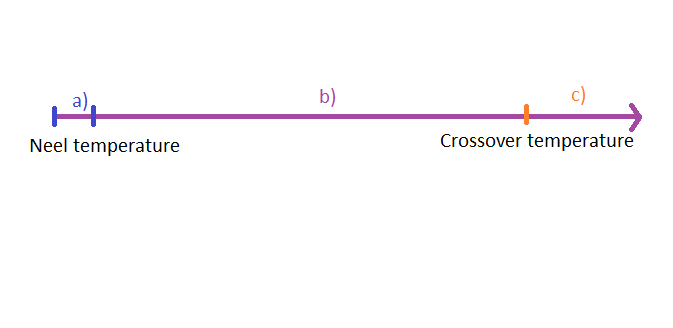
\includegraphics[scale=.50]{temperature.png}
\caption{Neel temperature and charging temperature are material dependent, yet the former tends to be in the sub Kelvin range and the latter tends to be in the thousands of Kelvin.}
\label{temperature}
\end{center}
\end{figure}

\subsection {Density of States in {\sc dias}}
The energy involved when removing or adding a particle to a lattice site is what determines the probability to jump to it. It then makes sense to ask what the distribution of potential energies will be. The purpose of this code was not originally to determine the density of energy states of an electron lattice. Nevertheless it serves two practical purposes. First, it helps to make sure that the particular energy contributions are balanced accordingly. Looking at the density of states, one can immediately associate characteristics to electrical potential, substrate potential, etc. Then, at a glance, one can quickly determine if the substrate potential is too strong and is washing out electric potential contributions. The second purpose is to assure that a particular system is fully relaxed before simulations begin. Due to the inherent randomness of the system, particular outcomes may sharply vary depending on the initial conditions. Assuring that the system is relaxed before starting can compensate for this. One clue that the system is relaxed is that in two dimensions, there will be a linear (absolute value) pattern near $0$ in the density of states. We use a previously determined algorithm in order to quickly relax our system ~\cite{Vinokur08}. We begin with a nearest-neighbor comparison of every particle site and moving them if the overall energy is lower. Then we find the particle which is imparting the most potential energy by existing. This is compared to the hole for which filling it would cause the most potential energy to be added to the system. If the two energies, when summed, are less than the original, then the switch is performed. The area around each switched particle is then scanned to see if any readjustments can be made to further lower the potential energy of the system. The density of states is then measured again everywhere and the process is repeated until the energy can no longer be reduced. The valley in the density of states can also be characterized. If the slope near $E=0$ is linear, then we know we are looking at a 2D system. If it is parabolic, then this signifies a 3D system. As a benchmark, we analyzed our valley slope and found it to agree with the 2D system characterization.


\subsection{Thoon Cluster and Computational Resources}
This research was performed on a variety of machines, mostly consisting of Nvidia graphics cards. I had access to one stand-alone pc with a GTX 570 graphics card, 8 pcs in a computer lab with GTX 570s, and 60 nodes with 2 GPU's each on the Gaea cluster in the computer science building. The Gaea cluster was powerful, but frequently busy such that only a third to an eighth was typically available. Meanwhile there was a computer lab with 8 linux based pcs, each with an Nvidia gtx 570. Unfortunately, they were barely on the same network. To remedy this, I wrote a script which divided up the parameter scans in the form of bash scripts and sent these to the respective computers. These then started the simulations and a timer in the form of a cron argument. The cron would then check every five minutes to see if the simulation was done. If so, then the data was sent back to the host computer. This had a few weaknesses, namely the clunkyness and the fact that one had to wait for the cron to trigger. This meant that short scans were impractical. Eventually this was all replaced with the free-lisence version of the Torque job scheduler. With the computers united into a small "cluster", running batches became more streamlined. This ad-hoc cluster is called THOON (Torque Hub On One Node). The cluster uses a network file system to share data in between the computers.

\section{Results}
\subsection{Algorithmic Benchmarking}
The average jump distance for a high temperature system should be ~0.69614 spaces. This matches to within $1\%$ accuracy with my results of 0.68943 spaces. This difference is negligible considering the statistical variation of any Monte Carlo system. The expected jump distance was found via Monte Carlo integrator. First, the values of Eq.~\ref{probability} were found at a grid of points with similar spacing to what we use in the simulation. Second, particles were dropped onto this grid depending on the function values a-la Monte Carlo method. Third, the mean jump distance was calculated via the first moment equation
\begin{eqnarray}
\bar r = \frac {\sum r \cdot n} {\sum n}, 
\label{firstMoment}
\end{eqnarray}
where $r$ is the distance from the center of the grid cell, and $n$ is the number of particles at each grid cell. The parameters for this comparison were fairly basic. The temperature was 1 degree kelvin, there was no external current, the system size was 100x100, and there was only one particle. Multiple particle comparisons have been done, but because the jump probabilities are different depending on wether the site is empty or full, the comparison becomes much more complicated. The point of this benchmark was to make sure the complicated GPU Monte-Carlo integrator was working as expected. With 3 major components to this system, (calculating the energies, calculating the weights from the energies, and calculating a jump site from the weights), this was a simple way to make sure everything was working together properly. Creating simple scripts to test more complicated scripts also became a useful tool in other parts of the research. For example, studying the behavior of the energy as a function of distance can be done via the Dias simulator, and outputs can be output for testing. But this can be complicated and the program may need to be changed and re-compiled in between tests. By writing a simple function in Octave and tuning the same parameters, the interaction between different energy sources could be observed more closely.

\subsection{Algorithmic Benchmarking}
The average jump distance for a high temperature system should be ~0.69614 spaces. This matches to within $1\%$ accuracy with my results of 0.68943 spaces. This difference is negligible considering the statistical variation of any Monte Carlo system. The expected jump distance was found via Monte Carlo integrator. First, the values of Eq.~\ref{probability} were found at a grid of points with similar spacing to what we use in the simulation. Second, particles were dropped onto this grid depending on the function values a-la Monte Carlo method. Third, the mean jump distance was calculated via the first moment equation
\begin{eqnarray}
\bar r = \frac {\sum r \cdot n} {\sum n}, 
\label{firstMoment}
\end{eqnarray}
where $r$ is the distance from the center of the grid cell, and $n$ is the number of particles at each grid cell. The parameters for this comparison were fairly basic. The temperature was 1 degree kelvin, there was no external current, the system size was 100x100, and there was only one particle. Multiple particle comparisons have been done, but because the jump probabilities are different depending on wether the site is empty or full, the comparison becomes much more complicated. The point of this benchmark was to make sure the complicated GPU Monte-Carlo integrator was working as expected. With 3 major components to this system, (calculating the energies, calculating the weights from the energies, and calculating a jump site from the weights), this was a simple way to make sure everything was working together properly. Creating simple scripts to test more complicated scripts also became a useful tool in other parts of the research. For example, studying the behavior of the energy as a function of distance can be done via the Dias simulator, and outputs can be output for testing. But this can be complicated and the program may need to be changed and re-compiled in between tests. By writing a simple function in Octave and tuning the same parameters, the interaction between different energy sources could be observed more closely.

\subsection{Fitting and Prediction}
  Other results also followed the expected trends. In Fig.~\ref{TvsRbar} , One can see that as the temperature rises, the system slowly kills any aditional help from the $E_{ij}$ component and it asymptotes to the jump distance related to the locality of the electron. In Fig.~\ref{JvsV} , The dependance of current on voltage is almost exponential. In Fig.~\ref{TvJ}, one can see how the electrons can't go as far once the temperature is increased. A modified version of the simulator was run to explore the physics of electron transport as the system becomes saturated. The number of electrons in the system was slowly increased and simulations were run at different numbers of particles. In ~\cite{Beloborodov07} they give approximate jump distances at various temperatures. We duplicated these and found similar values for $\bar \mu = .01$ and $\delta xy = .45$.

\begin{figure}[htbp]
\begin{center}
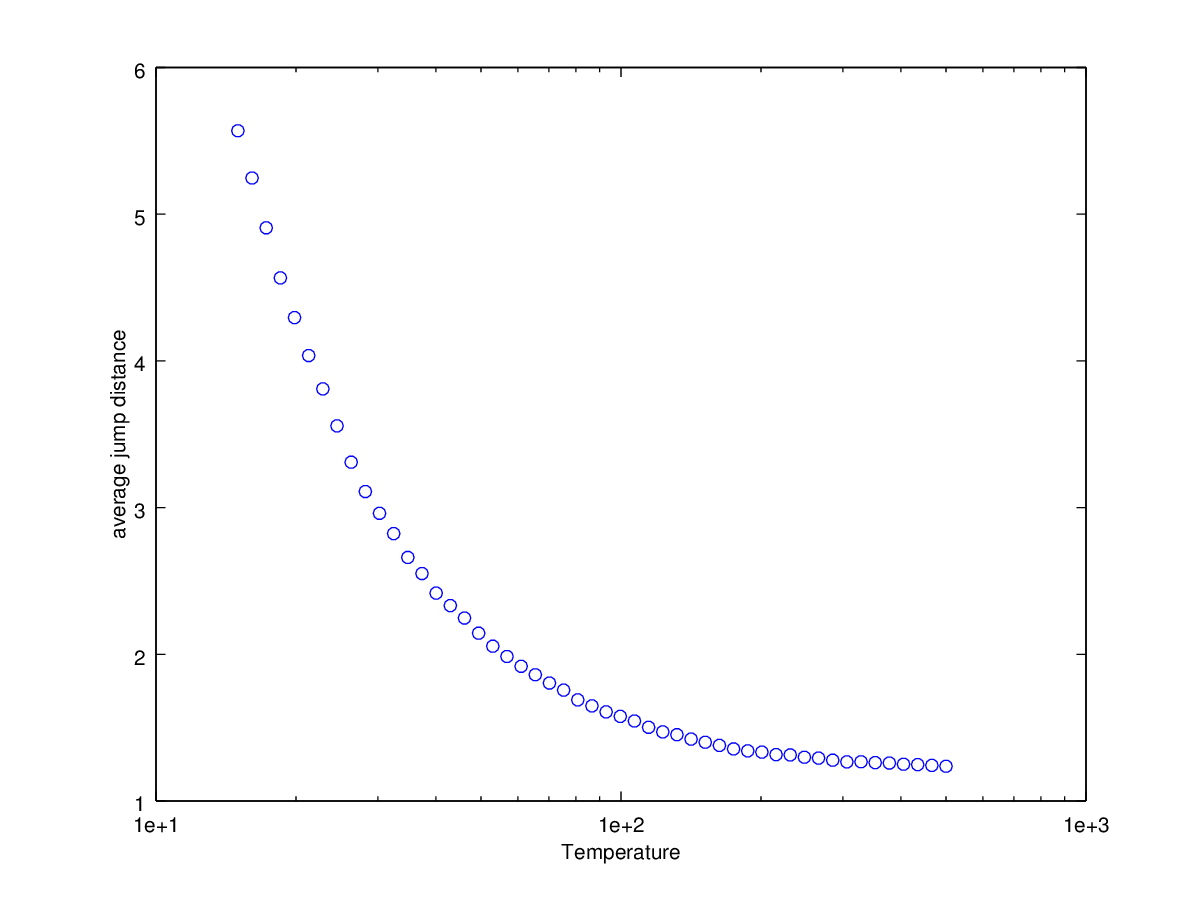
\includegraphics[scale=.50]{TvRGreat.png}
\caption{Temperature vs average jump distance .}
\label{TvsRbar}
\end{center}
\end{figure}

\begin{figure}[htbp]
\begin{center}
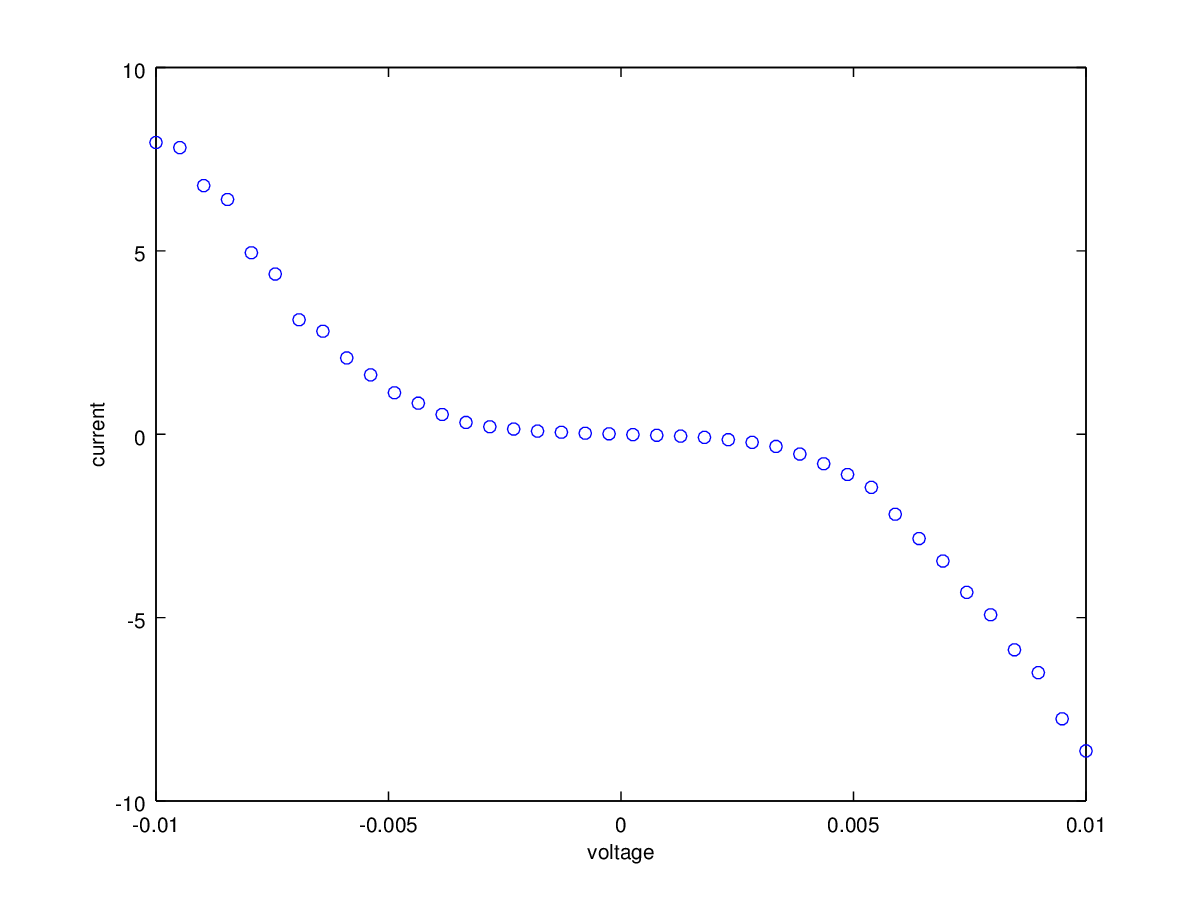
\includegraphics[scale=.50]{VvJGreat.png}
\caption{Current vs Voltage .}
\label{JvsV}
\end{center}
\end{figure}

\begin{figure}[htbp]
\begin{center}
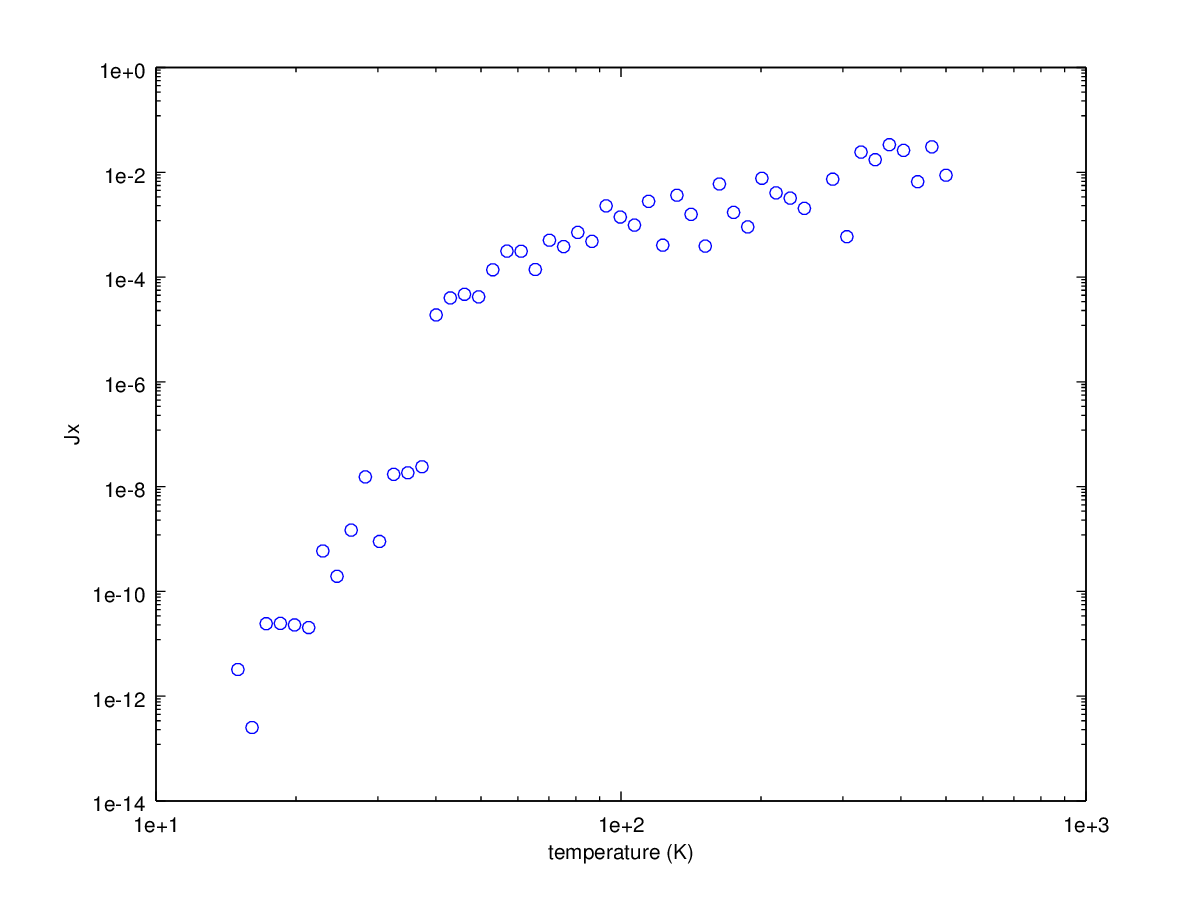
\includegraphics[scale=.50]{JvsT.png}
\caption{Temperature vs current .}
\label{TvJ}
\end{center}
\end{figure}

\begin{figure}[htbp]
\begin{center}
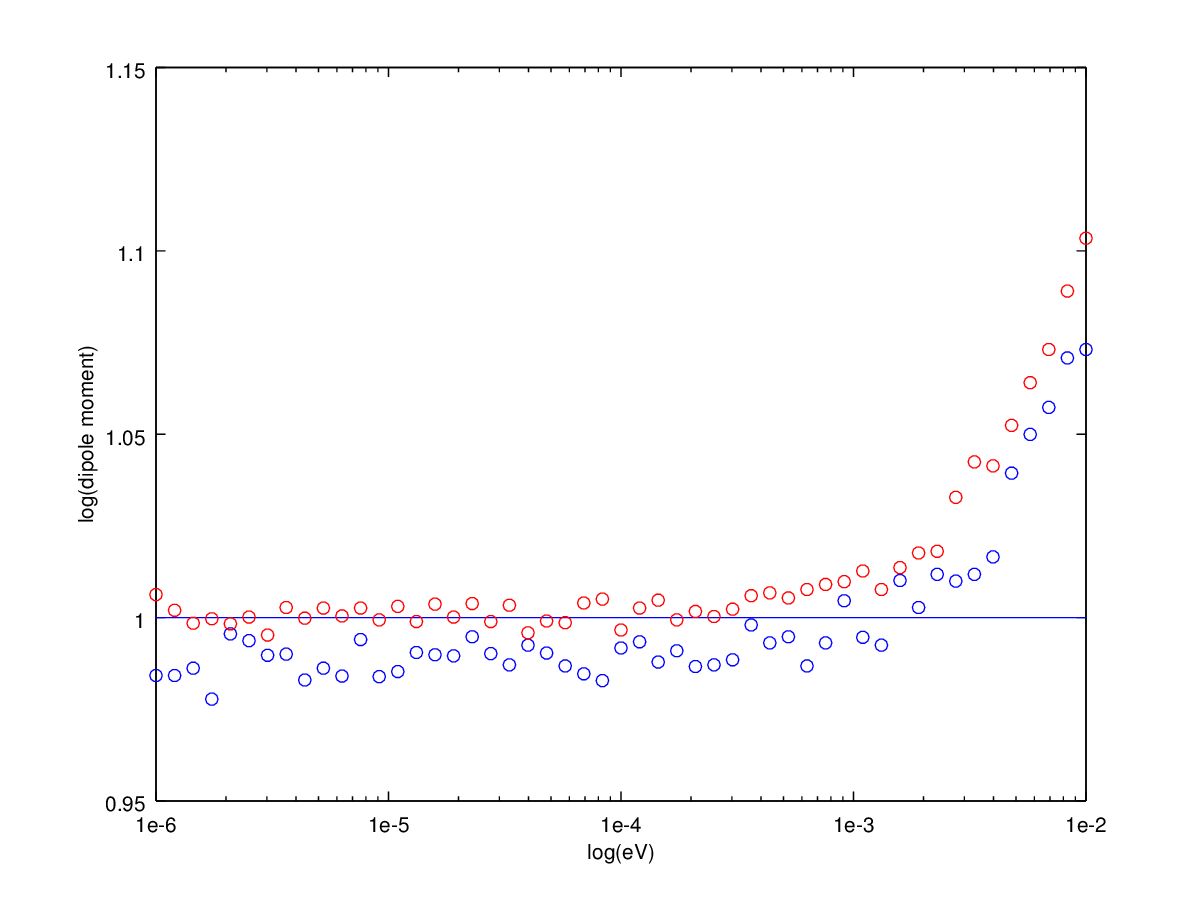
\includegraphics[scale=.50]{VoltageVsDipole.png}
\caption{This is a plot of the voltage vs the dipole moment of the electrons. The red dots are for a system without a temperature gradient. The blue dots are for a system with a temperature gradient. When the dipole moment becomes 0, the thermal force is pushing with as much strength aas the electric force. Using the Seebeck equation, we can estimate the Seebeck coefficient to be $10 \mu$}
\label{TvJ}
\end{center}
\end{figure}

To conclude, we have designed and implemented a conserved order parameter Markov Chain Monte Carlo continuous time algorithm. We benchmarked it and found it to have the correct relations between temperature, average jump distance, current, and voltage. We then used it to predict seebeck effects for different combinations of dielectric constants.
